% !TEX program = xelatex
\documentclass[12pt,hyperref,a4paper,UTF8]{ctexart}
\usepackage{CityUhomework}
\usepackage{float}

%%------------------Beginning of the text-----------------%%
\begin{document}

%%-----------------Cover------------------%%
\cover
\thispagestyle{empty}% Home page does not show page numbers


%%-----------------Catalog-------------------%%
\newpage
\tableofcontents

%%-----------------Main text starts here-------------------%%
\newpage
\section{题目}

\subsection{}

1. 下面关于串的的叙述中,正确的是(A)
\begin{enumerate}[A.]
    \item 串是一种特殊的线性表
    \item 串中的元素只能是字母
    \item 空串就是空白串
    \item 串的长度必须大于0
\end{enumerate}

\subsection{}
2. 两个字符串相等的条件是(D)
\begin{enumerate}[A.]
    \item 串的长度相等
    \item 含有相同的字符集
    \item 都是非空串
    \item 两个串的长度相等且对应位置的字符相同
\end{enumerate}

\subsection{}
3. 若串str = “ Software ”, 其子串的个数是(D)
\begin{enumerate}[A.]
    \item 8
    \item 9
    \item 36
    \item 37
\end{enumerate}

\subsection{}
4. 设有两个串p 和q, 其中是p的子串,则求q在p中首次出现位置的算法称为(C)
\begin{enumerate}[A.]
    \item 求子串
    \item 串联接
    \item 模式匹配
    \item 求串长
\end{enumerate}

\subsection{}
5. 串是一种特殊的线性表,其特殊性体现在(B)
\begin{enumerate}[A.]
    \item 可以顺序存储
    \item 数据元素是一个字符
    \item 可以链式存储
    \item 数据元素可以是多个字符
\end{enumerate}

\subsection{}

6. 若模式串T= “ababaa”, 求该模式串的Next 数组。
\begin{lstlisting}[style=CStyle]
    #include <stdio.h>
    #include <stdlib.h> 
    
    void computeNextArray(const char *pattern, int *next, int length)
    {
        int i = 0, j = -1;
        next[0] = -1; // 初始化第一个元素
    
        while (i < length - 1)
        {
            if (j == -1 || pattern[i] == pattern[j])// 如果j=-1或者pattern[i]等于pattern[j],则递增i和j,然后将next[i]赋值为j
            {
                i++;
                j++;
                next[i] = j;
            }
            else// 否则,将j赋值为next[j]
            {
                j = next[j];
            }
        }
    }
    
    int main()
    {
        const char *pattern = "ababaa";
        int length = 6;                                  // 模式串的长度
        int *next = (int *)malloc(length * sizeof(int)); // 动态分配内存
    
        computeNextArray(pattern, next, length);
    
        printf("Next array: ");
        for (int i = 0; i < length; i++)
        {
            printf("%d ", next[i]);
        }
        printf("\n");
    
        free(next); // 释放内存
    
        return 0;
    }
    
    
\end{lstlisting}

\begin{figure}[H]
    \centering
    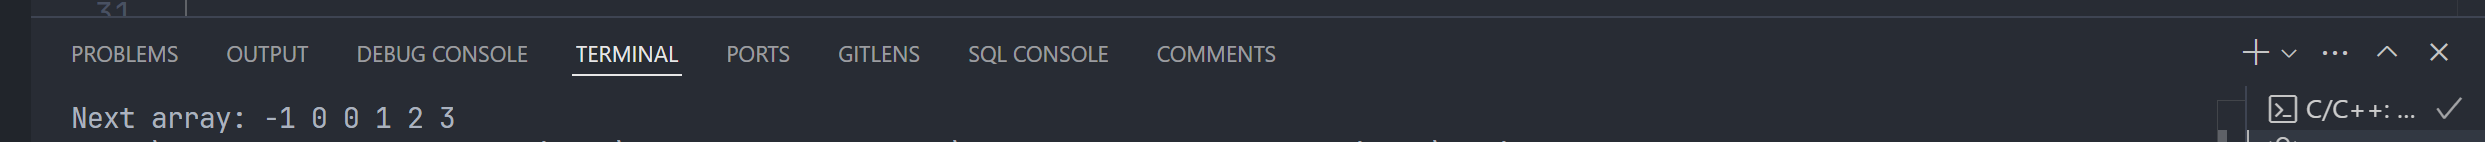
\includegraphics[width=0.8\textwidth]{figures/fig1.png}
    \caption{运行结果}
\end{figure}

\end{document}
